\chapter{Event simulation}
\label{chapter:MCsimulation}

The precise comparison of observed data with the theoretical predictions is necessary to quantify the consistency with the SM or some of its possible extensions. The simulation of the physics processes and the interaction of particles with the detector is therefore needed to model the expected contributions from different background or signal sources. Computer programs known as Monte Carlo (MC) event generators are able to simulate events from defined physics processes. Pseudo-random numbers are used to simulate individual events reproducing on average the predicted distributions. Finally MC techniques are also used to simulate the interaction of particles with the detector materials and the read-out of the detector.

This chapter presents an overview of the simulation of \pp\ collisions, followed by a description of the MC generators used for the analyses in this dissertation and the ATLAS detector simulation.

\section{Simulation of \pp\ collisions}
\label{sec:pp_simulation}
The simulation of \pp\ collisions requires the description of physics processes involving very different energy scales. From the high-energy scales present in the deep-inelastic scattering between the partons in the protons, to the very low-energy scales of the final state when the partons evolve into stable hadrons. In this soft regime the physics involved can not be described by perturbative QCD, making a full analytic description of the process impossible.
%The simulation of proton collisions has an additional difficulty, since protons are not elementary particles. At high energies though, the partons inside the proton behave as asymptotically free, and the hard interaction can be described as a parton-parton collision.

Fortunately, a key aspect in the simulation of \pp\ collisions is the possibility of factorizing the different energy scales involved in the process. The simulation of the hard interaction can be computed up to a fixed order in perturbation theory, while the description of the softer scales can be done with phenomenological models.

The simulation of the full \pp\ collision can be therefore factorized into different steps. 
First, the modeling of the partons inside the proton can be separated from the actual interaction. Two of these partons can then collide and undergo an interaction with a large momentum transfer.
Given the high-energy scale of the interaction, it can be computed at fixed order in perturbation theory.
Since the partons involved in the collision are color charged they will emit gluons, which in turn radiate further gluons or split into quark/anti-quark pairs, leading to the formation of parton showers.
The radiation process continues until the partons reach an energy scale of $Q \approx \unit[1]{\gev}$. At this stage hadronization takes place, and partons recombine into colorless hadrons. Phenomenological models are used to describe the hadronization process as well as the decay of hadrons into the final state particles that interact with the detector.
The different steps involved in the simulation are illustrated in figure~\ref{fig:MCexample}.

\begin{figure}[!t]
  \centering
  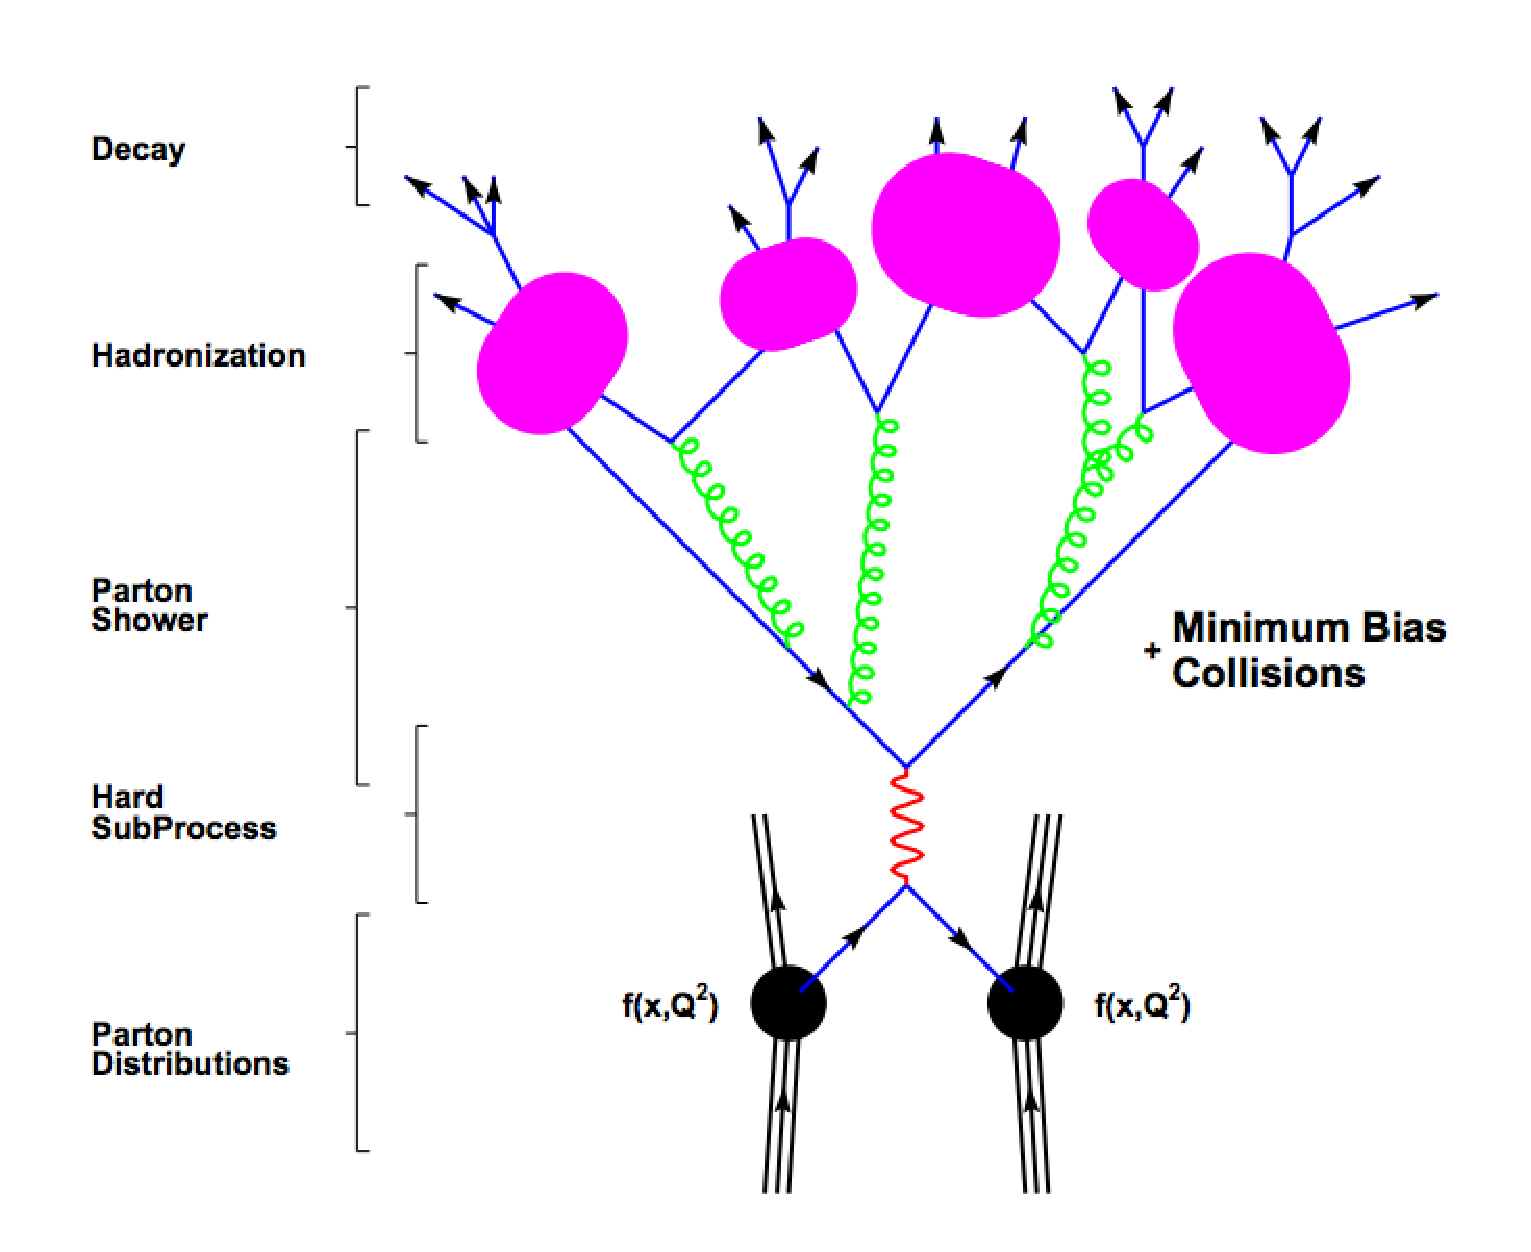
\includegraphics[width=0.7\textwidth]{MCsimulation/Figures/MCexample.eps}
  \caption{Representation of the different steps involved in the simulation of a \pp\ collision.}
  \label{fig:MCexample}
\end{figure}

\subsection{Factorization theorem}
The \xsec\ for a hadron collision producing a final state $X$, illustrated in figure~\ref{fig:hardscatter}, can be factorized into short- and long-distance effects delimited by a factorization scale, $\mu_F$, according to the factorization theorem~\cite{Collins:1989gx}:
\begin{equation}
  \sigma_{\pp \rightarrow X} = \sum_{a,b} \int dx_a dx_b\ f_a\left(x_a,\mu_F^2\right) f_b\left(x_b,\mu_F^2\right) \ \hat{\sigma}_{ab \rightarrow X}\left(x_a p_a,x_b p_b,\mu_F^2,\mu_R^2\right)~,
  \label{eq:factorization_theorem}
\end{equation}
where the sum runs over the parton types that can initiate the process.
%where $x_{i}$ is the fraction of momentum carried by the colliding parton  within the proton $p_{i}$, $f_{i}$ are the PDFs of each interacting parton, the sum runs over all parton types, and $\hat{\sigma}_{ab \rightarrow X}$ is the parton \xsec\ for incoming partons with momenta $p_{i} = x_{i} p_{i}$
The parton density function (PDF), $f_{i}\left(x_{i},\mu_F^2\right)$, encodes the probability of finding a parton of type $i$ within the proton, carrying a fraction of the proton's momentum $x_{i}$. 
PDFs are universal since they don't depend on the particular process. They are usually measured combining information from deep-inelastic scattering experiments and hadron colliders.

The \xsec\ for the partonic process $\hat{\sigma}_{ab \rightarrow X}\left(x_a p_a,x_b p_b,\mu_F^2,\mu_R^2\right)$ is computed explicitly at a fixed order in perturbation theory, which introduces a dependence on a renormalization scale $\mu_R$, that is usually chosen to be equal to $\mu_F$.
This step is also referred to as Matrix Element (ME) calculation, because it involves the calculation of the scattering matrix relating the initial and final state particles of the process.

\begin{figure}[!h]
  \begin{center}

    \myskip\begin{fmffile}{fmfhardscatter}
\unitlength=1mm
  \begin{center}
  \begin{fmfgraph*}(80,45)
    \fmfleft{P1,P2} \fmfright{P11,vv,P22}
    \fmf{fermion,tension=1,lab=$p_b$}{P1,g1}
    \fmf{fermion,tension=1,lab=$p_a$}{P2,g2}
    \fmfblob{.08w}{g1}
    \fmfblob{.08w}{g2}
    \fmf{plain,lab.side=left,lab=$x_bp_b$}{g1,v}
    \fmf{plain,lab.side=left,lab=$x_ap_a$}{v,g2}
    \fmf{dashes}{v,vv}
    \fmf{fermion}{g1,P11}
    \fmf{fermion}{g2,P22}
    \fmfv{lab.dist=.02w,lab=p}{P1}
    \fmfv{lab.dist=.02w,lab=p}{P2}
    \fmfv{lab.dist=.06w,lab.side=left,lab=$f_b(x_b)$}{g1}
    \fmfv{lab.dist=.06w,lab.side=left,lab=$f_a(x_a)$}{g2}
    \fmfv{decor.shape=circle,decor.filled=empty, decor.size=0.20w,lab.side=left,lab.dist=-0.35w,lab=$\hat{\sigma}(x_a,,x_b,,s)$}{v}
    \fmfv{lab=X}{vv}
    \fmffreeze
    \renewcommand{\P}[3]{\fmfi{plain}{%
        vpath(__#1,__#2) shifted (thick*(#3))}}
    \P{P1}{g1}{0,1}  \P{P1}{g1}{0,-1}
    \P{P2}{g2}{0,1}  \P{P2}{g2}{0,-1}
    \P{g1}{P11}{0,1} \P{g1}{P11}{0,-1}
    \P{g2}{P22}{0,1} \P{g2}{P22}{0,-1}
  \end{fmfgraph*}
  \end{center}
\end{fmffile}
\myskip
            %\myskip\input{fmfhardscatter}\myskip
%                \includegraphics[width=0.5\textwidth]{MCsimulation/Figures/hardscatter.png}
    \caption{Diagram of a generic hard scattering process. The partons, extracted from the colliding pp pair,
      carry a momentum fraction with respect to the proton energy described by a parton distribution function.
    The scattering of the partons is computed perturbatively and hence the kinematic properties of the final state object $X$ are predicted. }
    \label{fig:hardscatter}
  \end{center}
\end{figure}


\subsection{Fixed order QCD: matrix elements}
Schematically, the all-orders \xsec\ for the production of $X + \mathrm{anything}$, (inclusive $X$ production, with $X$ an arbitrary final state) can be expressed in the following way:
\begin{equation}
\hat{\sigma}_{ab\rightarrow X} \sim \underbrace{\sum_{k=0}^{\infty}{\int{d\Phi_{X+k}}}}_{\Sigma\text{ legs}}
                                          |\underbrace{\sum_{\ell=0}^{\infty}{\mathcal{M}^{\ell}_{X+k}} }_{\Sigma \text{ loops}}|^2~,
\label{eq:AllOrdersXSection}
\end{equation}
where the sum over $k$ represents the sum over additional ``real emission'' corrections (legs), and the sum over $\ell$ represents the sum over additional virtual corrections (loops).
$\Phi_{X+k}$ represents the phase space of the configuration with $k$ legs.

The various fixed-order truncations of a perturbative QCD calculation can be recovered by limiting the nested sums in equation~\ref{eq:AllOrdersXSection} to include only specific values of $k+\ell$:

\begin{itemize}
\item $k=0$, $\ell=0$: Leading order for inclusive $X$ production.
\item $k=n$, $\ell=0$: Leading order for $X+n$~jets.
\item $k+\ell \leq n$: N$^n$LO for $X$ (includes N$^{n-1}$LO for $X+1$ jet,  N$^{n-2}$LO for $X+2$ jets, and so on up to LO for $X+n$ jets).
\end{itemize}

Figure~\ref{fig:tt_jets} shows an example of several Feynman diagrams for a \ttbar\ final state at tree level ($k=0$, $\ell=0$), first emission ($k=1$, $\ell=0$) and including a virtual correction ($k=0$, $\ell=1$).
\begin{figure}[t!]
  \centering
  \begin{subfigure}{0.32\textwidth}
  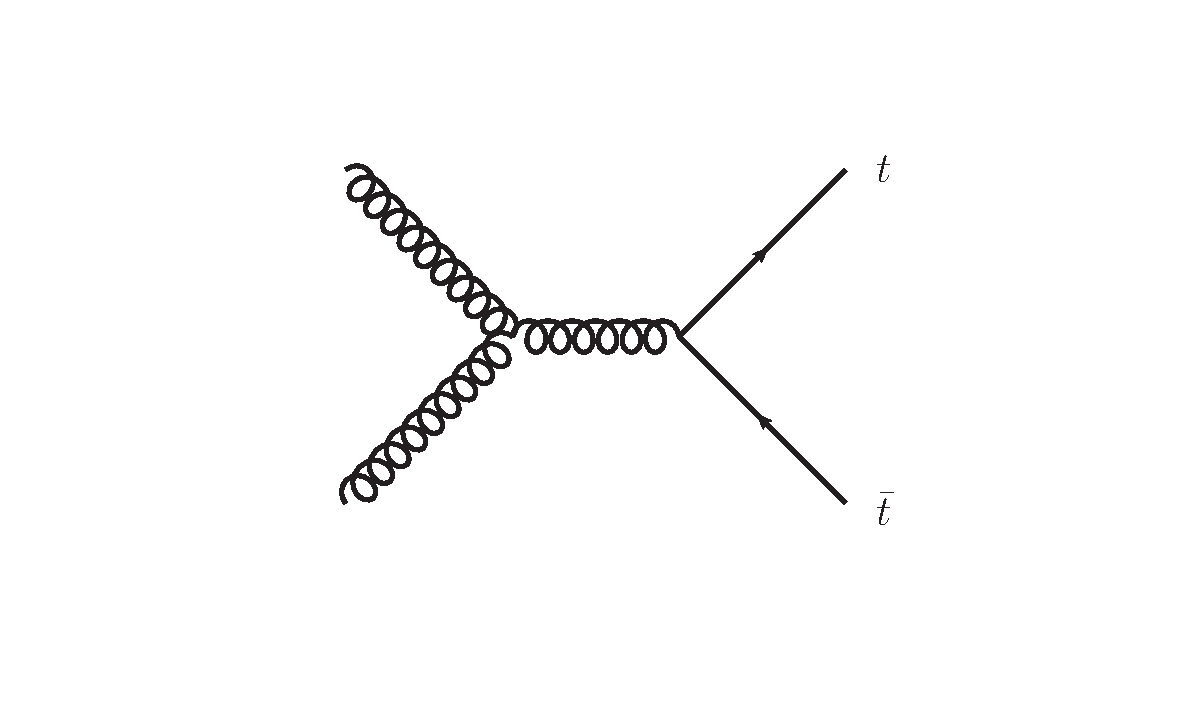
\includegraphics[width=\textwidth]{MCsimulation/Figures/tt_0jet}
  \caption{}\end{subfigure}
  \begin{subfigure}{0.32\textwidth}
  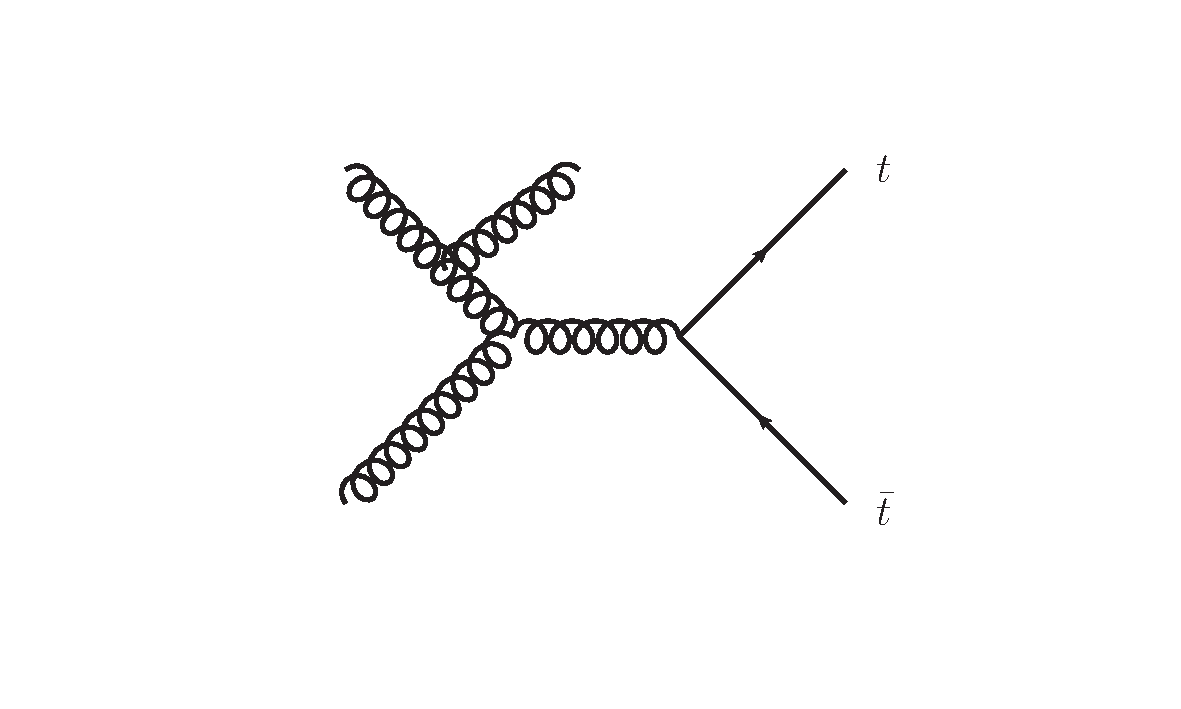
\includegraphics[width=\textwidth]{MCsimulation/Figures/tt_1jet}
  \caption{}\end{subfigure}
  \begin{subfigure}{0.32\textwidth}
  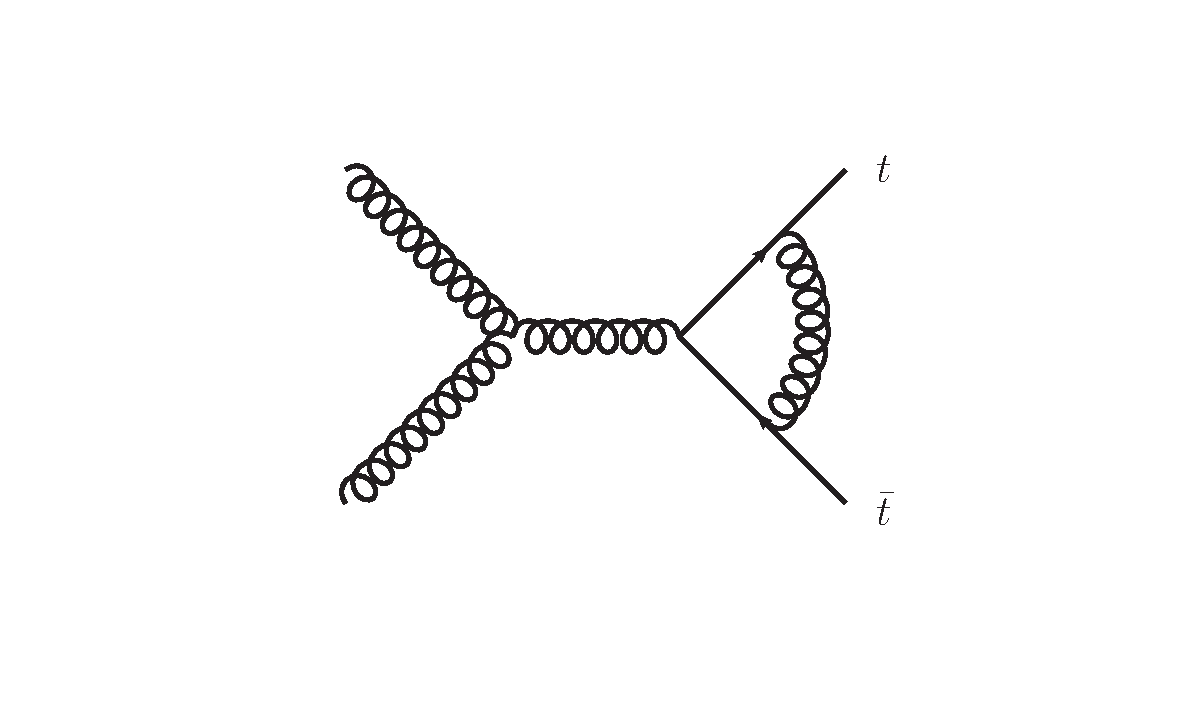
\includegraphics[width=\textwidth]{MCsimulation/Figures/tt_1loop}
  \caption{}\end{subfigure}
  \caption{Example Feynman diagrams of \ttbar\ production for (a) leading order, (b) first real emission and (c) first virtual correction.}
  \label{fig:tt_jets}
\end{figure}

The KLN theorem~\cite{KLN1,KLN2} states that the divergences originated in the loops exactly cancel against those from the real emissions, order by order in perturbation theory.
However, in a fixed-order calculation, e.g. leading order, in the situation for which $k\geq1$, $\ell=0$, the integration over the full momentum phase space will include configurations in which one or more of the $k$ partons become collinear or soft, thus leading to singularities in the integration region.
For this reason, the integration region needs to be modified to include only ``hard, well-separated'' momenta.
The remaining part of the phase space is then considered by the parton shower generators.

\subsection{Parton Shower}

Parton showers are included in the MC simulations to approximately account for the rest of higher order contributions to emulate a complete final state.
A parton shower generator simulates the successive emission of quarks and gluons from the partons in the final (or initial) state.
This simulation is approximate, since it assumes completely independent parton emissions and does not consider virtual corrections.
In the almost-collinear splitting of a parton, the $n+1$-parton differential \xsec\ can be related to the $n$-parton \xsec\ before splitting as:
\begin{equation}
  d\sigma_{n+1} \approx d\sigma_n~dP_i(z,q^2) \approx d\sigma_n~\frac{\alpha_S}{2\pi}\frac{dq^2}{q^2}dz~P_{ji}(z)~,
  \label{eq:splitting}
\end{equation}
where $dP_i(z,q^2)$ is the probability that parton $i$ will split into two partons at a virtuality scale or invariant mass $q^2$, with parton $j$ carrying a fraction $z$ of the momentum of parton $i$. An illustration of this process is given in figure~\ref{fig:splitting}.
\begin{figure}[t!]
  \centering
  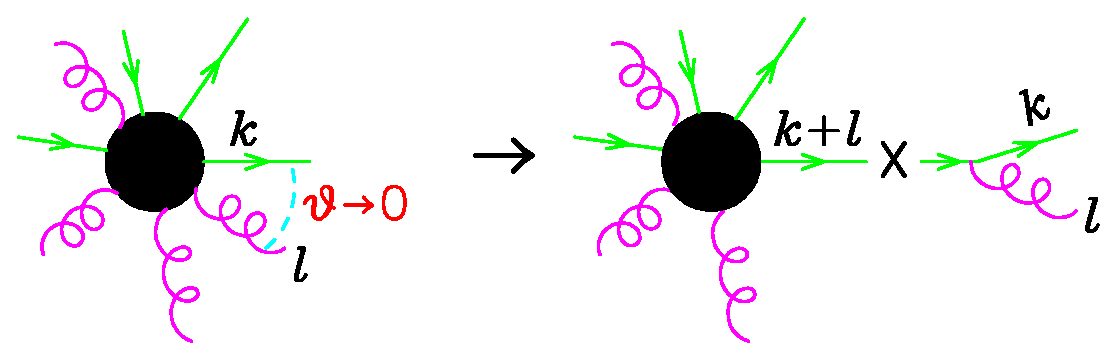
\includegraphics[width=0.7\textwidth]{MCsimulation/Figures/factorization}
  \caption{Representation of an $n+1$-parton process described as a splitting from an $n$-parton process.}
  \label{fig:splitting}
\end{figure}
%and $\phi$ are the opening angle and azimuthal angle of the splitting, and $P_i$ is the splitting function, which describes the distribution of the fraction $z$ of energy of the original parton, assigned to the new parton. 
There are three possible processes for QCD emission (splitting): $q \rightarrow gq$, $g \rightarrow gg$ and $g \rightarrow \qqbar$.
The simulation algorithm develops the shower by applying equation~\ref{eq:splitting} iteratively, for each parton involved in the hard interaction.

The implementation of the parton shower in MC programs is done via the Sudakov form factors:
\begin{equation}
  \Delta_i(q_1^2,q_2^2) = \text{exp} \left( - \sum_j \int_{q_2^2}^{q_1^2} \int_{z_{\text{min}}}^{z_{\text{max}}}  dP_i(z,q^2) \right)~.
  \label{eq:sudakov}
\end{equation}
The Sudakov form factors represent the probability that a parton evolves from an initial scale $q_1$ to a lower scale $q_2$ without splitting.

In final-state showers, the branching algorithm operates in the following steps:
\begin{enumerate}
  \item Given the initial scale $Q^2$, partons emit radiation at a scale $q_2$ determined by sampling equation~\ref{eq:sudakov}.
\item If the scale $q_2^2$ is below the hadronization scale, $q_2^2 < Q_0^2 \approx \unit[1]{\gev^2}$,  the shower development is terminated and hadronization takes place.
\item  Otherwise, the procedure is repeated for each new parton produced by the splitting, taking $q_2^2$ as initial scale.
\end{enumerate}

In the case of initial-state showers, the radiation is emitted by the colliding partons, and the final energy scale is the one entering the hard interaction. MC generators implement a \textit{backward evolution} that starts by setting the correct parton momentum for the hard scatter, and then develops the shower backwards, with ancestor partons gaining energy at each emission.

\subsection{Matrix element and parton shower matching}
The simplest fixed-order ME calculation is the LO one, $k=0$ and $l=0$ as represented in equation~\ref{eq:AllOrdersXSection}. However the precision of the pure LO calculation is often not sufficient for an accurate description of the final state. In this case multi-leg LO ($k \geq 1$, $l=0$) or N$^n$LO calculations ($k+l = n$) can be used, although with an infrared cut-off to prevent divergences from soft and collinear emissions. 
A problem arises when adding the parton shower evolution, since a double counting of certain phase space regions is present. A given final state with one additional emission is generated as both the ME term for $X+1$ parton, and in the first radiation of the parton shower starting from the $X+0$ parton state.

To remove this overlap, the phase space covered by the ME calculation, and the space covered by the parton-shower evolution needs to be separated. The procedure to distinguish between hard and large-angle emissions, described by the ME, and soft and collinear emissions, described by the PS, is referred to as ME-PS \textit{matching}.
The most widely-used matching schemes are the Catani-Krauss-Kuhn-Webber (CKKW \cite{Catani:2001cc}) and the Michelangelo L. Mangano (MLM \cite{Mangano:2006rw}) algorithms.

In the CKKW algorithm, a parton branching history is generated using the \kt algorithm \cite{Catani:1991hj}, given a configuration with $n$ partons in the final state.
The values of $\alpha_s$ in every vertex of the branching, and the Sudakov factor from every line between the vertices, are used to reweight the ME.
The initial conditions of the shower are then set to have a smooth transition between the reweighted ME and the parton shower, where the hard emissions in the shower evolution are vetoed if they have enough transverse momentum to produce a separate jet, according to the \kt algorithm.

The MLM algorithm starts by separating the events in exclusive samples of $n$ partons in the final state, on which the parton shower is added.
The parton configuration after the showering is then processed with a cone jet algorithm, with a radius $R_{\text{jet}}$.
The original $n$ partons are matched to the jets if $\Delta R(\text{jet}, \text{parton}) < R_{\text{jet}}$.
If all the partons are matched to a jet and there are no extra jets, i.e. $N_{\text{jets}}=n$, the event is accepted.
Otherwise, the event is rejected to avoid further hard emissions that would lead to additional jets.
Finally, the events with different jet multiplicities, $n=0, 1, 2, \ldots, k$, are recombined in a single sample.
The events in the sample with highest parton multiplicity $k$ are accepted if $N_\text{jets}\geq k$.

\subsection{Hadronization}
    \label{subsec:HadronizationModels}
As the partons evolve and radiate, the values of the shower evolution scale $Q^2$ decrease bringing the parton virtuality below the hadronization scale $Q_0^2 \approx \unit[1]{\gev}$. The confining effects of QCD become important and the dynamics enter a non-perturbative phase which leads to the formation of the observed final-state hadrons.
Event generators have to rely on phenomenological models based on general features of QCD.
The most used hadronization models are the string fragmentation and the cluster hadronization models, illustrated in figure~\ref{fig:HadronizationModels}.

In the string model~\cite{Andersson:1983ia,Sjostrand:1984ic}, the confinement between partons induced by the color force is represented by a gluonic string. For a quark-antiquark pair, as the color charges move apart, the string is stretched, and its potential energy grows. When the energy becomes of the order of hadron masses, it becomes energetically favorable for the string to break and create a new quark-antiquark pair. The two segments of string will stretch and break again, until all the energy has been converted into quark-antiquark pairs connected by short strings.

The cluster model~\cite{Webber:1983if,Marchesini:1987cf} relies on groupings of partons to form colorless clusters, after forcing the final state gluons to split into quark-antiquark pairs. The heaviest clusters can decay and split into smaller clusters. Most clusters will have masses below \unit[3]{\gev}, and their decay into hadrons is simulated with three-body models with intermediate resonances.

\begin{figure}[!t]
  \begin{center}
    \begin{subfigure}{0.3\textwidth}
        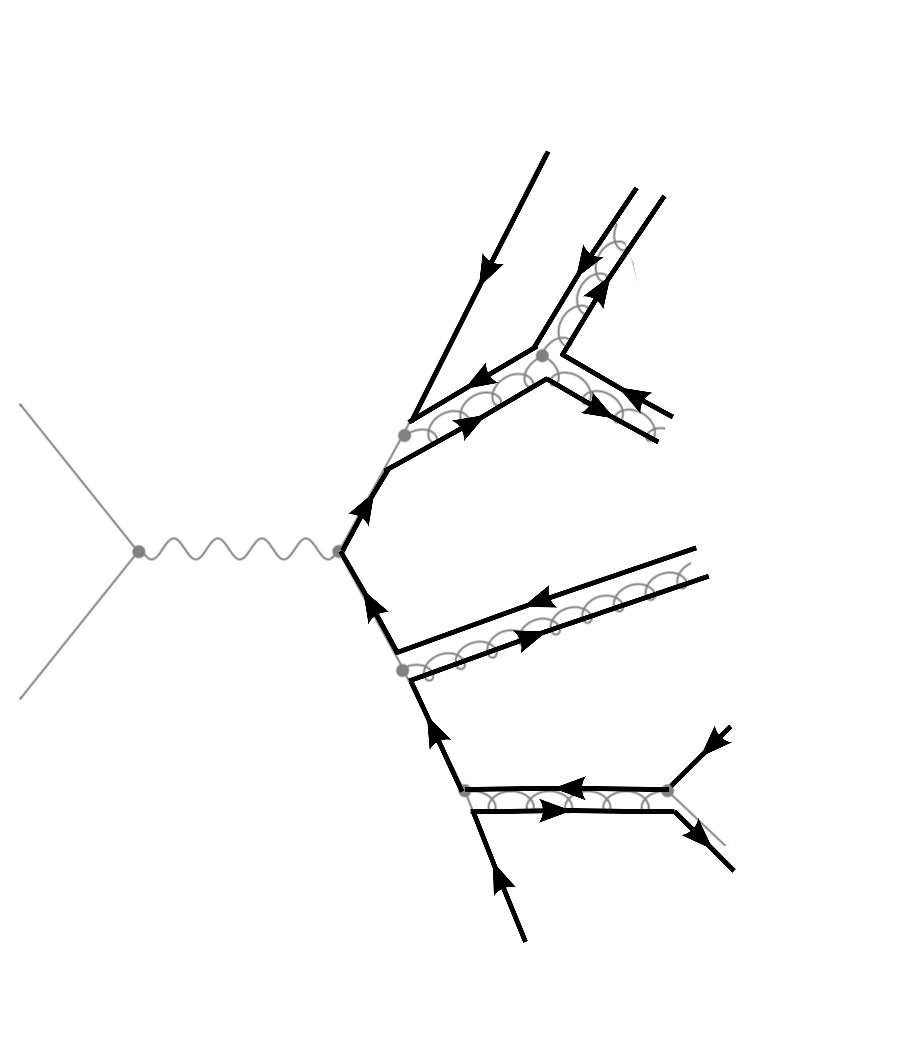
\includegraphics[width=\textwidth]{MCsimulation/Figures/had_colorflow.eps}
        \caption{}\end{subfigure}
    \begin{subfigure}{0.3\textwidth}
        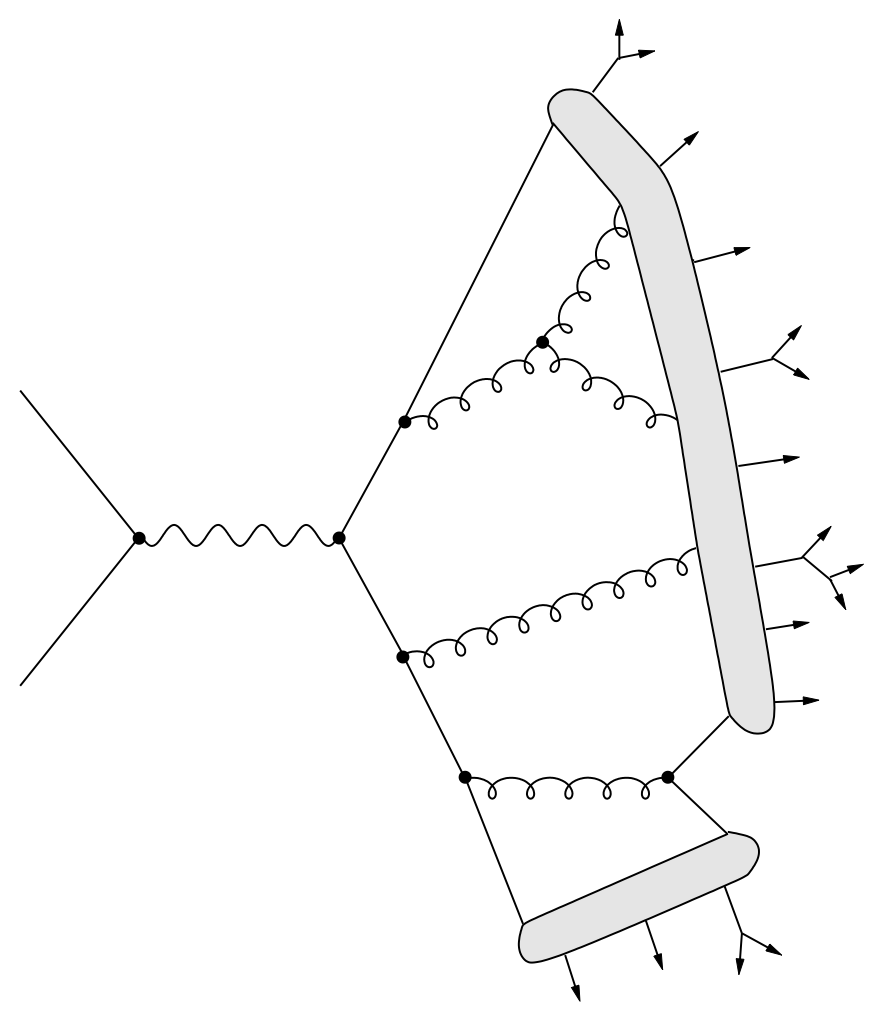
\includegraphics[width=\textwidth]{MCsimulation/Figures/HadronizationString.eps}
        \caption{}\end{subfigure}
    \begin{subfigure}{0.3\textwidth}
        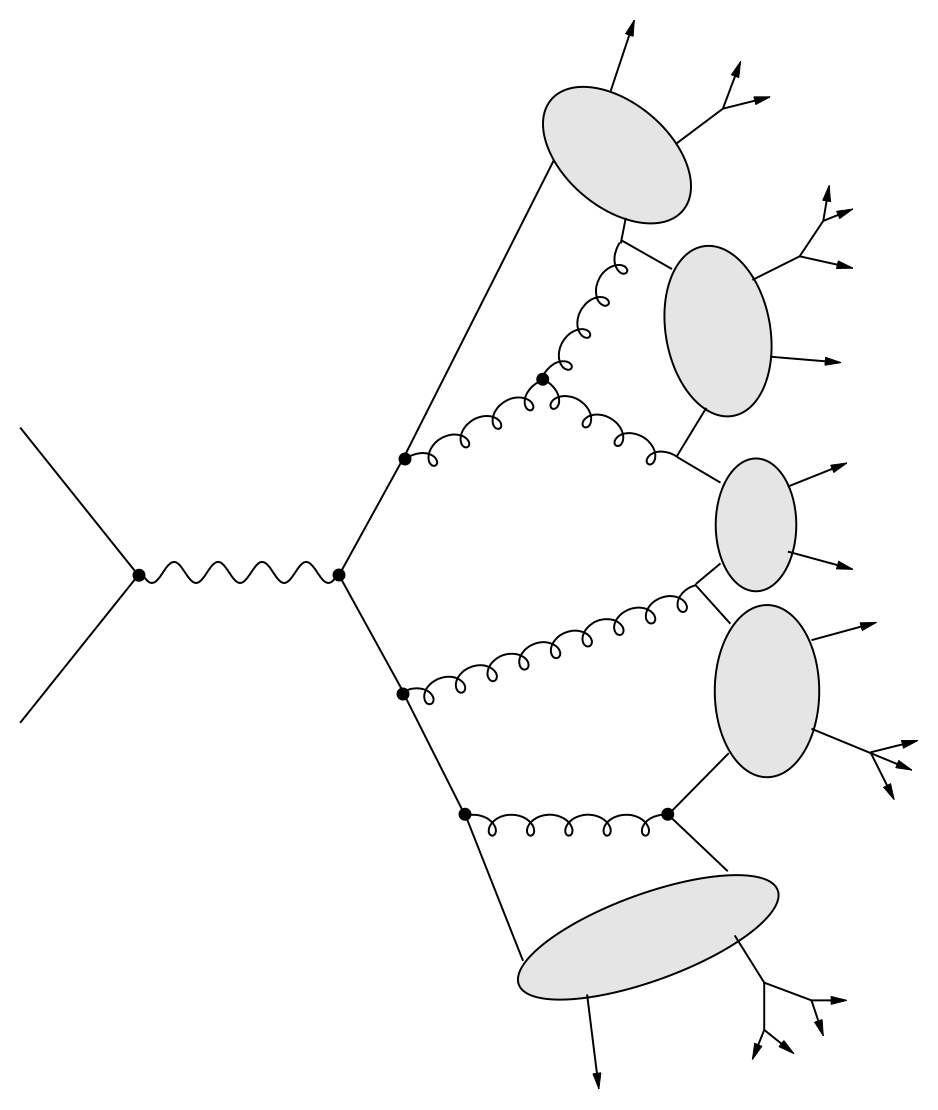
\includegraphics[width=\textwidth]{MCsimulation/Figures/HadronizationCluster.eps}
        \caption{}\end{subfigure}
  \end{center}
  \caption[Illustration of different hadronization models.]{Illustration of (a) the color flow in a given parton configuration and the models of (b) string fragmentation and (c) cluster hadronization.}
  \label{fig:HadronizationModels}
\end{figure}


\subsection{Underlying event}
The underlying event (UE) refers to the soft interactions involving spectator partons from the colliding protons. Because of the low energy scale of these processes, phenomenological models have to be used, where the parameters are tuned based on experimental data~\cite{Aad:2014hia}, such as the charged particle density (see figure~\ref{fig:UE}).
The large \xsec\ for gluon-gluon scattering makes multiple gluon scatterings per proton collision very likely. For this reason the generic soft scattering of partons is referred to as multiple parton interactions (MPI). The color connection with the beam remnants that are not interacting is also simulated with phenomenological models~\cite{Sjostrand:2006za,jimmy}.

\begin{figure}[!ht]
  \begin{center}
        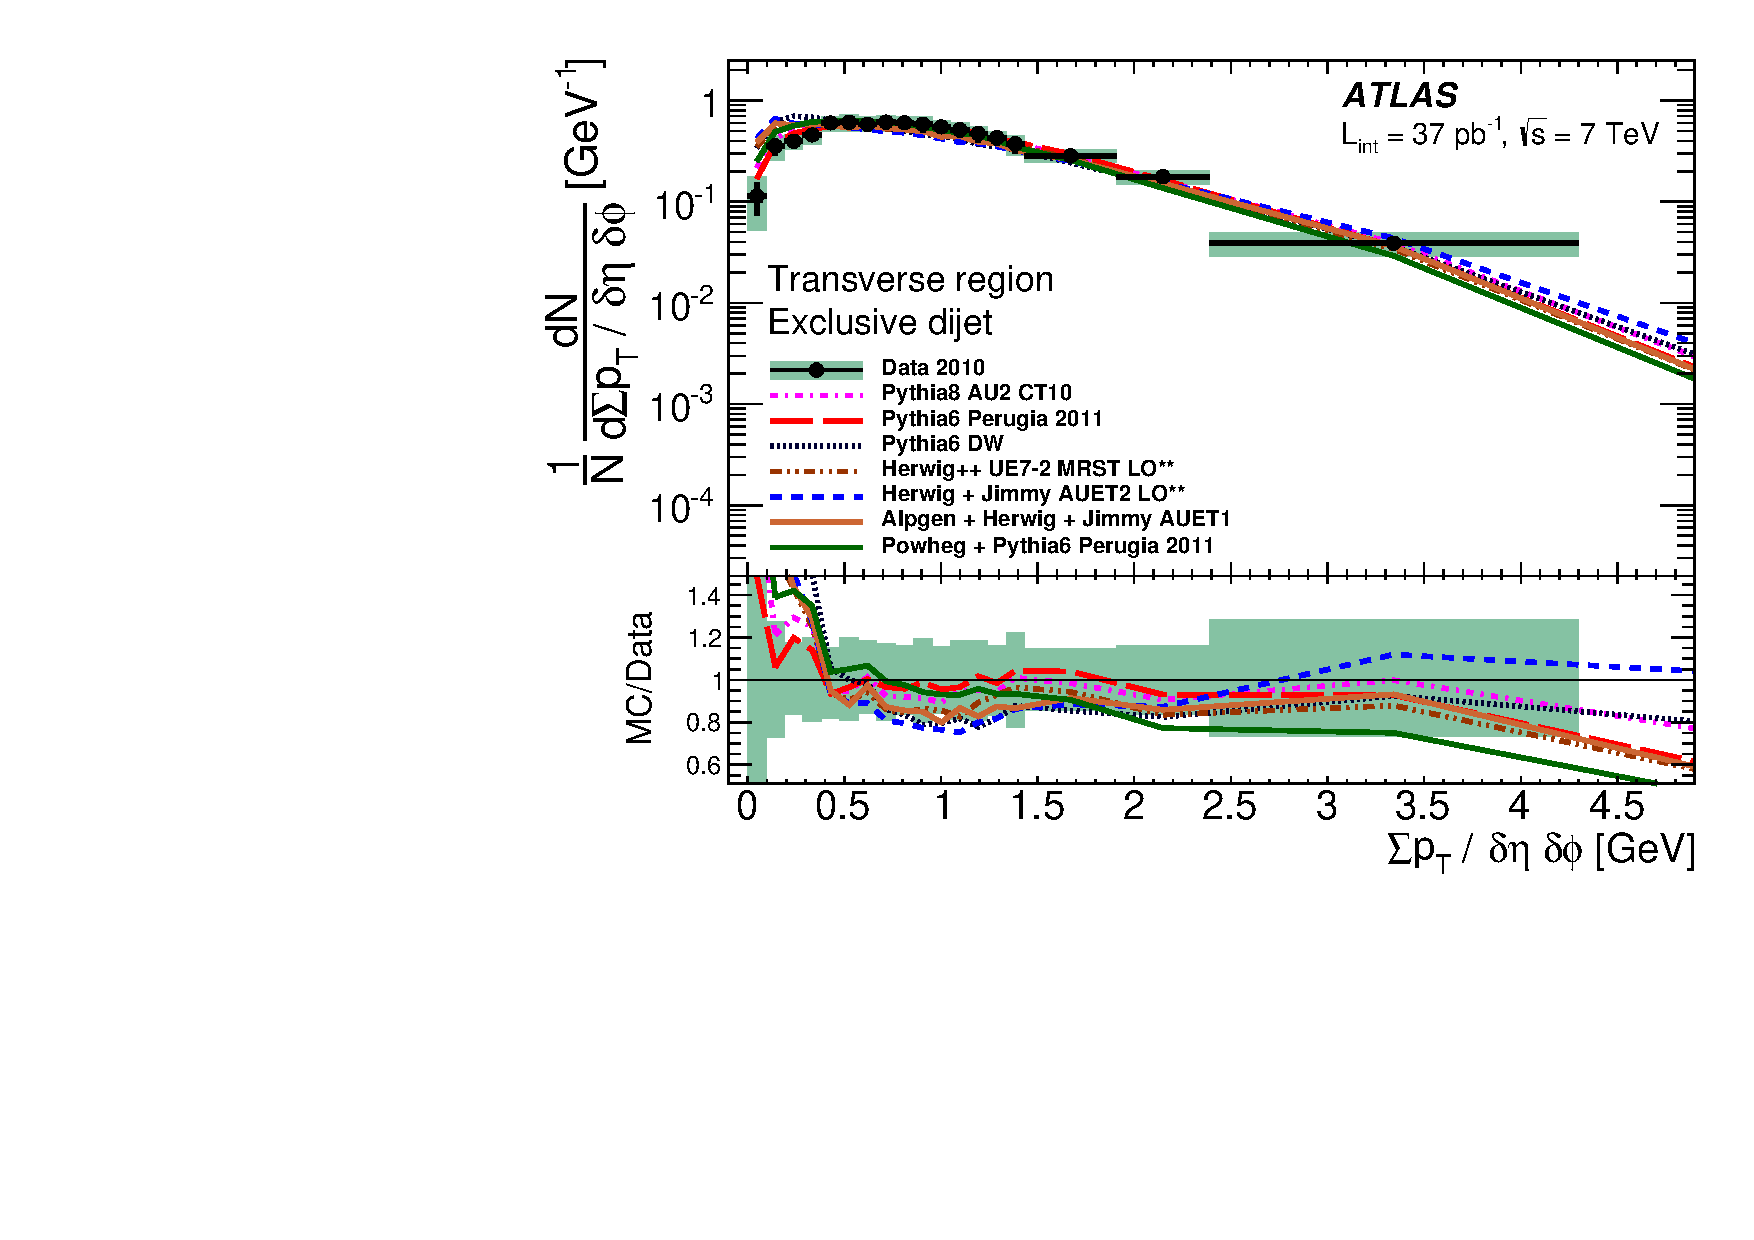
\includegraphics[width=0.7\textwidth]{MCsimulation/Figures/figaux_04b}
  \end{center}
  \caption{Normalized charged-particle \pt\ sum density distributions in ATLAS data compared to different underlying event models. From reference~\cite{Aad:2014hia}.}
  \label{fig:UE}
\end{figure}
\subsection{\Pileup}
In-time \pileup\ events are originated from the scattering of protons in the same bunch of the hadron generating the hard process of interest. They mainly consist of soft QCD interactions and are modeled in a similar way as the UE. Out-of-time \pileup\ is modeled with the same physics process, but considering interactions in past bunch crossings and simulating the time response of the readout electronics.

\section{Monte Carlo generators}
\label{sec:MCgenerators}
Different Monte Carlo generators are used for the description of different physics processes of relevance. Generators can be classified as either multi-purpose generators, capable of performing the full simulation chain, or ME generators which have to be interfaced with an additional parton shower.

\subsection{General purpose Monte Carlo generators}
\begin{description}
  \item[\pythia~\cite{Sjostrand:2006za}] is a multi-purpose MC generator using LO calculations for $2 \rightarrow n$ ($n \leq 3$) processes and PS with emissions ordered in transverse momentum. The Lund string model is used for hadronization, and UE simulation is included.
  \item[\herwig~\cite{Corcella:2000bw}]  is a multi-purpose MC generator using LO calculations for $2 \rightarrow 2$ processes and PS with emissions ordered in opening angle. The cluster model is used for hadronization and for the UE description. \herwig\ is typically interfaced with the standalone software \jimmy~\cite{Butterworth:1996zw} that simulates UE and MPI.
\end{description}

\subsection{Multi-leg leading-order generators}
\begin{description}
\item[\alpgen~\cite{Mangano:2002ea}] is a MC generator providing LO calculations of $2 \rightarrow n$ ($n \leq 9$) processes. It can be interfaced with either \pythia\ or \herwig\ for parton shower evolution, hadronization and UE modeling. ME-PS matching is applied with the MLM algorithm.
\item[\madgraph~\cite{Alwall:2011uj}] is a MC generator specialized in the computation of ME involving $2 \rightarrow n$ ($n \leq 6$) processes at LO. It is interfaced with \pythia\ for the parton shower evolution and the ME-PS matching is performed with the MLM algorithm.
\item[\sherpa~\cite{Gleisberg:2008ta}] is a MC generator that can provide multi-leg leading-order calculations. It contains its own parton shower algorithm based on the Catani-Seymour dipole formalism~\cite{Schumann:2007mg}. The ME-PS matching is implemented with an improved version of the CKKW algorithm~\cite{Hoeche:2009rj}.
\end{description}

\subsection{NLO generators}
\begin{description}
  \item[\powheg~\cite{Frixione:2007vw}] is an event generator computing ME at NLO in perturbative QCD. \powheg\ can be interfaced with either \pythia\ or \herwig\ for the modeling of the parton shower, hadronization and UE. 
  \item[\sherpa] can also generate events at NLO after being interfaced with additional libraries to compute the loop amplitudes. \sherpa\ in conjunction with \OpenLoops~\cite{Cascioli:2011va} is used to model the \ttbb\ process at NLO, which is the largest background for the analyses discussed in this dissertation.
\end{description}

\section{ATLAS simulation}
\label{sec:ATLASsim}
The final output of the MC generators is a list of four-vectors of all stable particles produced in the event, after decay and hadronization of the intermediate unstable particles. This output can be used in order to study the physics processes at the \textit{particle level}. In order to compare it with the recorded data, the MC has to be analyzed after the reconstruction in the detector, i.e. at the \textit{reconstruction level}. The detector simulation software, \Geant~\cite{G4}, models the interaction of the particles with the detector. The simulation of the interaction converts the energy deposits into electronic signals taking into account the geometry, materials and readout system of the ATLAS detector.
A less refined simulation, known as Atlfast-II or AF2~\cite{AF2}, is also available. This reduces considerably the CPU time necessary to process the events by applying a parameterized description of the particle showers in the calorimeters.

Figure~\ref{fig:reco_flow} shows the ATLAS simulation data flow with the different steps of the MC and data processing.

\begin{figure}[hbt!]
  \begin{center}
  	\includegraphics[width=0.9\textwidth]{MCsimulation/Figures/outline_v3} %v2 without the color lines
	\caption{The flow of the ATLAS simulation software, from event generators (top left) through reconstruction (top right).
        The red path leads to {\it particle level} physics objects, the blue path to
        {\it reconstructed level} physics objects, while the green path shows the real data
        flow to physics objects.
        %Algorithms are placed in square-cornered boxes and persistent data objects are placed in rounded boxes. 
        %The optional pile-up portion of the chain, used only when events are overlaid, is dashed. 
        %Generators are used to produce data in HepMC format.  
        %Monte Carlo truth is saved in addition to energy depositions in the detector (hits). 
        SDO stands for Simulated Data Object, ROD for Read Out Driver~\cite{Aad:2010ah}.}
\label{fig:reco_flow}
\end{center}
\end{figure}

%The \Geant\ parameters are tuned using test-beam and \pp\ collision data. The accuracy of the detector simulation is based on the information from the geometry database, which contains the description of the detector volumes in terms of dimensions, geometry, position and material composition, while the conditions database provides the information on the detector real-time conditions like dead channels, misalignments, or temperatures. Since conditions vary from run to run, it is important that the detector simulation reproduces as close as possible the real status of ATLAS during a particular data-taking period. %rewrite
%

\section{Monte Carlo corrections}
\label{sec:mcweights}

Monte Carlo samples are corrected to reproduce the best known theoretical \xsec,
usually NLO or NNLO, even when they are produced with a lower order MC generator.
In addition to the normalization to the recorded luminosity, the events are weighted
to match the expected number of interactions per bunch crossing $\left<\mu\right>$
 in real data-taking conditions. 

To ensure an accurate modeling of the detector effects in the reconstruction and identification efficiencies $\varepsilon$, the efficiencies in MC are corrected with multiplicative scale factors. The scale factors are defined as:
\begin{equation}
  SF = \frac{\varepsilon_{\rm data}}{\varepsilon_{\rm MC}}
  \label{eq:SF}
\end{equation}
where $\varepsilon_{\rm data}$ and $\varepsilon_{\rm MC}$ are measured in dedicated data calibration samples and in the equivalent MC simulation, respectively. Analogously, energy scale and resolution of the different physics objects in the simulation are corrected to match the corresponding measurements in data.

\clearpage
\bibliographystyle{Bibliography/atlasnote}
\bibliography{Bibliography/myBib}
